

%🍁% \chapter{Dictionaries  |  字典}
\chapter{字典}

%🍁% This chapter presents another built-in type called a dictionary.
%🍁% Dictionaries are one of Python's best features; they are the
%🍁% building blocks of many efficient and elegant algorithms.

本章介绍另一个内建数据类型: {\em 字典} (dictionary)。
字典是 Python 中最优秀的特性之一; 许多高效、优雅的算法以此为基础。

%🍁% \section{A dictionary is a mapping  |  字典即映射}
\section{字典即映射}

\index{dictionary}  \index{dictionary}
\index{type!dict}  \index{key}
\index{key-value pair}  \index{index}

%🍁% A {\bf dictionary} is like a list, but more general.  In a list,
%🍁% the indices have to be integers; in a dictionary they can
%🍁% be (almost) any type.

{\em 字典} 与列表类似, 但是更加通用。
在列表中, 索引必须是整数;但在字典中, 它们可以是(几乎)任何类型。

%🍁% A dictionary contains a collection of indices, which are called {\bf
%🍁%   keys}, and a collection of values.  Each key is associated with a
%🍁% single value.  The association of a key and a value is called a {\bf
%🍁%   key-value pair} or sometimes an {\bf item}.  \index{item}

字典包含了一个索引的集合, 被称为 {\em 键} (keys) , 和一个 {\em 值} (values)的集合。   一个键对应一个值。   这种一一对应的关联被称为 {\em 键值对} (key-value pair) ,  有时也被称为 {\em 项} (item) 。

%🍁% In mathematical language, a dictionary represents a {\bf mapping}
%🍁% from keys to values, so you can also say that each key
%🍁% ``maps to'' a value.
%🍁% As an example, we'll build a dictionary that maps from English
%🍁% to Spanish words, so the keys and the values are all strings.

在数学语言中, 字典表示的是从键到值的 {\em 映射}, 所以你也可以说每一个键 ``映射到'' 一个值。    举个例子, 我们接下来创建一个字典, 将英语单词映射至西班牙语单词, 因此键和值都是字符串。

%🍁% The function {\tt dict} creates a new dictionary with no items.
%🍁% Because {\tt dict} is the name of a built-in function, you
%🍁% should avoid using it as a variable name.

\li{dict} 函数生成一个不含任何项的新字典。   由于 \li{dict} 是内建函数名, 你应该避免使用它来命名变量。

\index{dict function}  \index{function!dict}

\begin{lstlisting}
>>> eng2sp = dict()
>>> eng2sp
{}
\end{lstlisting}

%🍁% The squiggly-brackets, \verb"{}", represent an empty dictionary.
%🍁% To add items to the dictionary, you can use square brackets:

花括号 \verb"{}" 表示一个空字典。  你可以使用方括号向字典中增加项:

\index{squiggly bracket}  \index{bracket!squiggly}

\begin{lstlisting}
>>> eng2sp['one'] = 'uno'
\end{lstlisting}

%
%🍁% This line creates an item that maps from the key
%🍁% \verb"'one'" to the value \verb"'uno'".  If we print the
%🍁% dictionary again, we see a key-value pair with a colon
%🍁% between the key and value:

这行代码创建一个新项, 将键 \li{'one'} 映射至值 \li{'uno'}。
如果我们再次打印该字典, 会看到一个以冒号分隔的键值对:

\begin{lstlisting}
>>> eng2sp
{'one': 'uno'}
\end{lstlisting}

%
%🍁% This output format is also an input format.  For example,
%🍁% you can create a new dictionary with three items:

输出的格式同样也是输入的格式。   例如, 你可以像这样创建一个包含三个项的字典:

\begin{lstlisting}
>>> eng2sp = {'one': 'uno', 'two': 'dos', 'three': 'tres'}
\end{lstlisting}

%
%🍁% But if you print {\tt eng2sp}, you might be surprised:

但是, 如果你打印 \li{eng2sp} , 结果可能会让你感到意外:

\begin{lstlisting}
>>> eng2sp
{'one': 'uno', 'three': 'tres', 'two': 'dos'}
\end{lstlisting}

%
%🍁% The order of the key-value pairs might not be the same.  If
%🍁% you type the same example on your computer, you might get a
%🍁% different result.  In general, the order of items in
%🍁% a dictionary is unpredictable.

键-值对的顺序和原来不同。
同样的例子在你的电脑上可能有不同的结果。  通常来说, 字典中项的顺序是不可预知的。

%🍁% But that's not a problem because
%🍁% the elements of a dictionary are never indexed with integer indices.
%🍁% Instead, you use the keys to look up the corresponding values:

但这没有关系, 因为字典的元素不使用整数索引来索引, 而是用键来查找对应的值:

\begin{lstlisting}
>>> eng2sp['two']
'dos'
\end{lstlisting}

%
%🍁% The key \verb"'two'" always maps to the value \verb"'dos'" so the order
%🍁% of the items doesn't matter.

键 \li{'two'} 总是映射到值 \li{'dos'} , 因此项的顺序没有关系。

%🍁% If the key isn't in the dictionary, you get an exception:

如果键不存在字典中, 会抛出一个异常:

\index{exception!KeyError}  \index{KeyError}

\begin{lstlisting}
>>> eng2sp['four']
KeyError: 'four'
\end{lstlisting}

%
%🍁% The {\tt len} function works on dictionaries; it returns the
%🍁% number of key-value pairs:

\li{len} 函数也适用于字典;它返回键值对的个数:

\index{len function}  \index{function!len}

\begin{lstlisting}
>>> len(eng2sp)
3
\end{lstlisting}

%
%🍁% The {\tt in} operator works on dictionaries, too; it tells you whether
%🍁% something appears as a {\em key} in the dictionary (appearing
%🍁% as a value is not good enough).

\li{in} 操作符也适用于字典;它可以用来检验字典中是否存在某个 {\em 键} (仅仅有这个值还不够)。

\index{membership!dictionary}  \index{in operator}
\index{operator!in}

\begin{lstlisting}
>>> 'one' in eng2sp
True
>>> 'uno' in eng2sp
False
\end{lstlisting}

%
%🍁% To see whether something appears as a value in a dictionary, you
%🍁% can use the method {\tt values}, which returns a collection of
%🍁% values, and then use the {\tt in} operator:

想要知道字典中是否存在某个值, 你可以使用 \li{values} 方法, 它返回值的集合, 然后你可以使用 \li{in} 操作符来验证:

\index{values method}  \index{method!values}

\begin{lstlisting}
>>> vals = eng2sp.values()
>>> 'uno' in vals
True
\end{lstlisting}

%
%🍁% The {\tt in} operator uses different algorithms for lists and
%🍁% dictionaries.  For lists, it searches the elements of the list in
%🍁% order, as in Section~\ref{find}.  As the list gets longer, the search
%🍁% time gets longer in direct proportion.

\li{in} 操作符对列表和字典采用不同的算法。
对于列表, 它按顺序依次查找目标, 如 \ref{find}~节 所示。
随着列表的增长, 搜索时间成正比增长。

%🍁% For dictionaries, Python uses an
%🍁% algorithm called a {\bf hashtable} that has a remarkable property: the
%🍁% {\tt in} operator takes about the same amount of time no matter how
%🍁% many items are in the dictionary.  I explain how that's possible
%🍁% in Section~\ref{hashtable}, but the explanation might not make
%🍁% sense until you've read a few more chapters.

对于字典, Python 使用一种叫做 {\em 哈希表} (hashtable) 的算法,
这种算法具备一种了不起的特性: 无论字典中有多少项,  \li{in} 运算符搜索所需的时间都是一样的。   我将在第二十一章的哈希表一节中具体解释背后的原理,
但是如果你不再多学习几章内容, 现在去看解释的话可能很难理解。

%🍁% \section{Dictionary as a collection of counters  |  字典作为计数器集合}
\section{字典作为计数器集合}
\label{histogram}
\index{counter}

%🍁% Suppose you are given a string and you want to count how many
%🍁% times each letter appears.  There are several ways you could do it:

假设给你一个字符串, 你想计算每个字母出现的次数。
有多种方法可以使用:

%🍁% \begin{enumerate}
%🍁%
%🍁% \item You could create 26 variables, one for each letter of the
%🍁% alphabet.  Then you could traverse the string and, for each
%🍁% character, increment the corresponding counter, probably using
%🍁% a chained conditional.
%🍁%
%🍁% \item You could create a list with 26 elements.  Then you could
%🍁% convert each character to a number (using the built-in function
%🍁% {\tt ord}), use the number as an index into the list, and increment
%🍁% the appropriate counter.
%🍁%
%🍁% \item You could create a dictionary with characters as keys
%🍁% and counters as the corresponding values.  The first time you
%🍁% see a character, you would add an item to the dictionary.  After
%🍁% that you would increment the value of an existing item.
%🍁%
%🍁% \end{enumerate}

\begin{enumerate}

\item 你可以生成26个变量, 每个对应一个字母表中的字母。  然后你可以遍历字符串, 对于 每个字符, 递增相应的计数器, 你可能会用到链式条件。

\item 你可以生成具有26个元素的列表。   然后你可以将每个字符转化为一个数字(使用内建函数 \li{ord} ), 使用这些数字作为列表的索引, 并递增适当的计数器。

\item 你可以生成一个字典, 将字符作为键, 计数器作为相应的值。  字母第一次出现时, 你应该向字典中增加一项。   这之后, 你应该递增一个已有项的值。

\end{enumerate}

%🍁% Each of these options performs the same computation, but each
%🍁% of them implements that computation in a different way.

每个方法都是为了做同一件事, 但是各自的实现方法不同。

\index{implementation}

%🍁% An {\bf implementation} is a way of performing a computation;
%🍁% some implementations are better than others.  For example,
%🍁% an advantage of the dictionary implementation is that we don't
%🍁% have to know ahead of time which letters appear in the string
%🍁% and we only have to make room for the letters that do appear.

{\em 实现} 是指执行某种计算的方法;有的实现更好。
例如, 使用字典的实现有一个优势, 即我们不需要事先知道字符串中有几种字母,
只要在出现新字母时分配空间就

%🍁% Here is what the code might look like:

代码可能是这样的:

\begin{lstlisting}
def histogram(s):
    d = dict()
    for c in s:
        if c not in d:
            d[c] = 1
        else:
            d[c] += 1
    return d
\end{lstlisting}

%
%🍁% The name of the function is {\tt histogram}, which is a statistical
%🍁% term for a collection of counters (or frequencies).

函数名叫 \li{histogram} (直方图) , 是计数器(或是频率)集合的统计术语。

\index{histogram}  \index{frequency}
\index{traversal}

%🍁% The first line of the
%🍁% function creates an empty dictionary.  The {\tt for} loop traverses
%🍁% the string.  Each time through the loop, if the character {\tt c} is
%🍁% not in the dictionary, we create a new item with key {\tt c} and the
%🍁% initial value 1 (since we have seen this letter once).  If {\tt c} is
%🍁% already in the dictionary we increment {\tt d[c]}.

函数的第一行生成一个空字典。   \li{for} 循环遍历该字符串。
每次循环, 如果字符 \li{c} 不在字典中,  我们用键 \li{c} 和初始值 \li{1} 生成一个新项 (因为该字母出现了一次)。   如果 \li{c} 已经在字典中了, 那么我们递增 \li{d[c]} 。

\index{histogram}

%🍁% Here's how it works:

下面是运行结果:

\begin{lstlisting}
>>> h = histogram('brontosaurus')
>>> h
{'a': 1, 'b': 1, 'o': 2, 'n': 1, 's': 2, 'r': 2, 'u': 2, 't': 1}
\end{lstlisting}

%
%🍁% The histogram indicates that the letters \verb"'a'" and \verb"'b'"
%🍁% appear once; \verb"'o'" appears twice, and so on.

\li{histogram} 函数表明字母 \li{'a'} 和 \li{'b'} 出现了一次,   \li{'o'} 出现了两次, 等等。

\index{get method}  \index{method!get}

%🍁% Dictionaries have a method called {\tt get} that takes a key
%🍁% and a default value.  If the key appears in the dictionary,
%🍁% {\tt get} returns the corresponding value; otherwise it returns
%🍁% the default value.  For example:

字典类有一个 \li{get} 方法, 接受一个键和一个默认值作为参数。
如果字典中存在该键, 则返回对应值;否则返回传入的默认值。   例如:

\begin{lstlisting}
>>> h = histogram('a')
>>> h
{'a': 1}
>>> h.get('a', 0)
1
>>> h.get('b', 0)
0
\end{lstlisting}

%
%🍁% As an exercise, use {\tt get} to write {\tt histogram} more concisely.  You
%🍁% should be able to eliminate the {\tt if} statement.

我们做个练习, 试着用 \li{get} 简化 \li{histogram} 函数。  你应该能够不再使用 \li{if} 语句。


%🍁% \section{Looping and dictionaries  |  循环和字典}
\section{循环和字典}

\index{dictionary!looping with}  \index{looping!with dictionaries}
\index{traversal}

%🍁% If you use a dictionary in a {\tt for} statement, it traverses
%🍁% the keys of the dictionary.  For example, \verb"print_hist"
%🍁% prints each key and the corresponding value:

在 \li{for} 循环中使用字典会遍历其所有的键。
例如, 下面的 \li{print_hist} 会打印所有键与对应的值:

\begin{lstlisting}
def print_hist(h):
    for c in h:
        print(c, h[c])
\end{lstlisting}

%
%🍁% Here's what the output looks like:

输出类似:

\begin{lstlisting}
>>> h = histogram('parrot')
>>> print_hist(h)
a 1
p 1
r 2
t 1
o 1
\end{lstlisting}

%
%🍁% Again, the keys are in no particular order.  To traverse the keys
%🍁% in sorted order, you can use the built-in function {\tt sorted}:

重申一遍, 字典中的键是无序的。
如果要以确定的顺序遍历字典, 你可以使用内建方法 \li{sorted}:

\index{keys method}  \index{method!keys}

\begin{lstlisting}
>>> for key in sorted(h):
...     print(key, h[key])
a 1
o 1
p 1
r 2
t 1
\end{lstlisting}

%TODO: get this on Atlas


%🍁% \section{Reverse lookup  |  逆向查找}
\section{逆向查找}
\label{raise}

\index{dictionary!lookup}  \index{dictionary!reverse lookup}
\index{lookup, dictionary}  \index{reverse lookup, dictionary}

%🍁% Given a dictionary {\tt d} and a key {\tt k}, it is easy to
%🍁% find the corresponding value {\tt v = d[k]}.  This operation
%🍁% is called a {\bf lookup}.

给定一个字典 \li{d} 以及一个键 \li{t} , 很容易找到相应的值 \li{v = d[k]} 。
该运算被称作 {\em 查找} (lookup) 。

%🍁% But what if you have {\tt v} and you want to find {\tt k}?
%🍁% You have two problems: first, there might be more than one
%🍁% key that maps to the value {\tt v}.  Depending on the application,
%🍁% you might be able to pick one, or you might have to make
%🍁% a list that contains all of them.  Second, there is no
%🍁% simple syntax to do a {\bf reverse lookup}; you have to search.

但是如果你想通过 \li{v} 找到 \li{k} 呢?
有两个问题:第一, 可能有不止一个的键其映射到值v。
你可能可以找到唯一一个, 不然就得用 \li{list} 把所有的键包起来。
第二, 没有简单的语法可以完成 {\em 逆向查找} (reverse lookup) ; 你必须搜索。

%🍁% Here is a function that takes a value and returns the first
%🍁% key that maps to that value:

下面这个函数接受一个值并返回映射到该值的第一个键:

\begin{lstlisting}
def reverse_lookup(d, v):
    for k in d:
        if d[k] == v:
            return k
    raise LookupError()
\end{lstlisting}

%
%🍁% This function is yet another example of the search pattern, but it
%🍁% uses a feature we haven't seen before, {\tt raise}.  The
%🍁% {\bf raise statement} causes an exception; in this case it causes a
%🍁% {\tt LookupError}, which is a built-in exception used to indicate
%🍁% that a lookup operation failed.

该函数是搜索模式的另一个例子, 但是它使用了一个我们之前没有见过的特性, \li{raise}。   \li{raise} 语句 能触发异常, 这里它触发了 \li{ValueError}, 这是一个表示查找操作失败的内建异常。

\index{search}  \index{pattern!search}
\index{raise statement} \index{statement!raise}
\index{exception!LookupError} \index{LookupError}

%🍁% If we get to the end of the loop, that means {\tt v}
%🍁% doesn't appear in the dictionary as a value, so we raise an
%🍁% exception.

如果我们到达循环结尾, 这意味着字典中不存在 \li{v} 这个值, 所以我们触发一个异常。

%🍁% Here is an example of a successful reverse lookup:

下面是一个成功逆向查找的例子:

\begin{lstlisting}
>>> h = histogram('parrot')
>>> key = reverse_lookup(h, 2)
>>> key
'r'
\end{lstlisting}

%
%🍁% And an unsuccessful one:

以及一个失败的例子:

\begin{lstlisting}
>>> key = reverse_lookup(h, 3)
Traceback (most recent call last):
  File "<stdin>", line 1, in <module>
  File "<stdin>", line 5, in reverse_lookup
LookupError
\end{lstlisting}

%
%🍁% The effect when you raise an exception is the same as when
%🍁% Python raises one: it prints a traceback and an error message.

你触发的异常和 Python 触发的产生效果一样:都打印一条回溯和错误信息。

\index{traceback}  \index{optional argument}
\index{argument!optional}

%🍁% The {\tt raise} statement can take a detailed error message as an
%🍁% optional argument.  For example:

\li{raise} 语句接受一个详细的错误信息作为可选的实参。    例如:

\begin{lstlisting}
>>> raise LookupError('value does not appear in the dictionary')
Traceback (most recent call last):
  File "<stdin>", line 1, in ?
LookupError: value does not appear in the dictionary
\end{lstlisting}

%
%🍁% A reverse lookup is much slower than a forward lookup; if you
%🍁% have to do it often, or if the dictionary gets big, the performance
%🍁% of your program will suffer.

逆向查找比正向查找慢得多; 如果你频繁执行这个操作或是字典很大, 程序性能会变差。

%🍁% \section{Dictionaries and lists  |  字典和列表}
\section{字典和列表}
\label{invert}

%🍁% Lists can appear as values in a dictionary.  For example, if you
%🍁% are given a dictionary that maps from letters to frequencies, you
%🍁% might want to invert it; that is, create a dictionary that maps
%🍁% from frequencies to letters.  Since there might be several letters
%🍁% with the same frequency, each value in the inverted dictionary
%🍁% should be a list of letters.

在字典中, 列表可以作为值出现。
例如, 如果你有一个从字母映射到频率的字典,  而你想倒转它;
也就是生成一个从频率映射到字母的字典。
因为可能有些字母具有相同的频率, 所以在倒转字典中的每个值应该是一个字母组成的列表。

\index{invert dictionary}  \index{dictionary!invert}

%🍁% Here is a function that inverts a dictionary:

下面是一个倒转字典的函数:

\begin{lstlisting}
def invert_dict(d):
    inverse = dict()
    for key in d:
        val = d[key]
        if val not in inverse:
            inverse[val] = [key]
        else:
            inverse[val].append(key)
    return inverse
\end{lstlisting}

%
%🍁% Each time through the loop, {\tt key} gets a key from {\tt d} and
%🍁% {\tt val} gets the corresponding value.  If {\tt val} is not in {\tt
%🍁%   inverse}, that means we haven't seen it before, so we create a new
%🍁% item and initialize it with a {\bf singleton} (a list that contains a
%🍁% single element).  Otherwise we have seen this value before, so we
%🍁% append the corresponding key to the list.  \index{singleton}

每次循环,  \li{key} 从 \li{d} 获得一个键和相应的值 \li{val} 。
如果 \li{val} 不在 \li{inverse} 中, 意味着我们之前没有见过它,
因此我们生成一个新项并用一个 {\em 单元素集合} (singleton) (只包含一个元素的列表)初始化它。   否则就意味着之前已经见过该值, 因此将其对应的键添加至列表。

%🍁% Here is an example:

举个例子:

\begin{lstlisting}
>>> hist = histogram('parrot')
>>> hist
{'a': 1, 'p': 1, 'r': 2, 't': 1, 'o': 1}
>>> inverse = invert_dict(hist)
>>> inverse
{1: ['a', 'p', 't', 'o'], 2: ['r']}
\end{lstlisting}

\begin{figure}
\centerline
{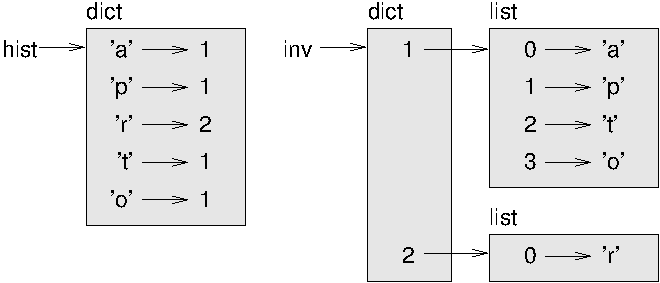
\includegraphics[scale=0.8]{../source/figs/dict1.pdf}}
\caption{State diagram.}
\label{fig.dict1}
\end{figure}

%🍁% Figure~\ref{fig.dict1} is a state diagram showing {\tt hist} and {\tt inverse}.
%🍁% A dictionary is represented as a box with the type {\tt dict} above it
%🍁% and the key-value pairs inside.  If the values are integers, floats or
%🍁% strings, I draw them inside the box, but I usually draw lists
%🍁% outside the box, just to keep the diagram simple.

图~\ref{fig.dict1} 是关于 \li{hist} 与 \li{inverse} 的状态图。  字典用标有类型 \li{dict} 的方框表示, 方框中是键值对。  如果值是整数、浮点数或字符串,
我就把它们画在方框内部, 但我通常把列表画在方框外面, 目的只是为了不让图表变复杂。

\index{state diagram}  \index{diagram!state}

%🍁% Lists can be values in a dictionary, as this example shows, but they
%🍁% cannot be keys.  Here's what happens if you try:

如本例所示, 列表可以作为字典中的值, 但是不能是键。
下面演示了这样做的结果:

\index{TypeError}  \index{exception!TypeError}

\begin{lstlisting}
>>> t = [1, 2, 3]
>>> d = dict()
>>> d[t] = 'oops'
Traceback (most recent call last):
  File "<stdin>", line 1, in ?
TypeError: list objects are unhashable
\end{lstlisting}

%
%🍁% I mentioned earlier that a dictionary is implemented using
%🍁% a hashtable and that means that the keys have to be {\bf hashable}.

我之前提过, 字典使用哈希表实现, 这意味着键必须是 {\bf 可哈希的} (hashable) 。

\index{hash function}  \index{hashable}

%🍁% A {\bf hash} is a function that takes a value (of any kind)
%🍁% and returns an integer.  Dictionaries use these integers,
%🍁% called hash values, to store and look up key-value pairs.


{\em 哈希} (hash) 函数接受一个值 (任何类型) 并返回一个整数。
字典使用被称作哈希值的这些整数, 来存储和查找键值对。
\index{immutability}

%🍁% This system works fine if the keys are immutable.  But if the
%🍁% keys are mutable, like lists, bad things happen.  For example,
%🍁% when you create a key-value pair, Python hashes the key and
%🍁% stores it in the corresponding location.  If you modify the
%🍁% key and then hash it again, it would go to a different location.
%🍁% In that case you might have two entries for the same key,
%🍁% or you might not be able to find a key.  Either way, the
%🍁% dictionary wouldn't work correctly.

如果键是不可变的, 那么这种实现可以很好地工作。
但是如果键是可变的, 如列表, 那么就会发生糟糕的事情。
例如, 当你生成一个键值对时, Python哈希该键并将其存储在相应的位置。
如果你改变键然后再次哈希它, 它将被存储到另一个位置。
在那种情况下, 对于相同的键, 你可能有两个值,  或者你可能无法找到一个键。
无论如何, 字典都不会正确的工作。

%🍁% That's why keys have to be hashable, and why mutable types like
%🍁% lists aren't.  The simplest way to get around this limitation is to
%🍁% use tuples, which we will see in the next chapter.

这就是为什么键必须是可哈希的, 以及为什么如列表这种可变类型不能作为键。
绕过这种限制最简单的方法是使用元组,  我们将在下一章中介绍。

%🍁% Since dictionaries are mutable, they can't be used as keys,
%🍁% but they {\em can} be used as values.

因为字典是可变的, 因此它们不能作为键, 但是 {\em 可以} 用作值。


%🍁% \section{Memos  |  备忘}
\section{备忘}
\label{memoize}

%🍁% If you played with the {\tt fibonacci} function from
%🍁% Section~\ref{one.more.example}, you might have noticed that the bigger
%🍁% the argument you provide, the longer the function takes to run.
%🍁% Furthermore, the run time increases quickly.

如果你在 \ref{one.more.example}节中接触过 \li{fibonacci} 函数,  你可能注意到输入的实参越大, 函数运行就需要越多时间。
而且运行时间增长得非常快。

\index{fibonacci function}  \index{function!fibonacci}

%🍁% To understand why, consider Figure~\ref{fig.fibonacci}, which shows
%🍁% the {\bf call graph} for {\tt fibonacci} with {\tt n=4}:

要理解其原因, 思考 图~\ref{fig.fibonacci} , 它展示了当 \li{n=4} 时 \li{fibonacci} 的 {\em 调用图} (call graph) :

\begin{figure}
\centerline
{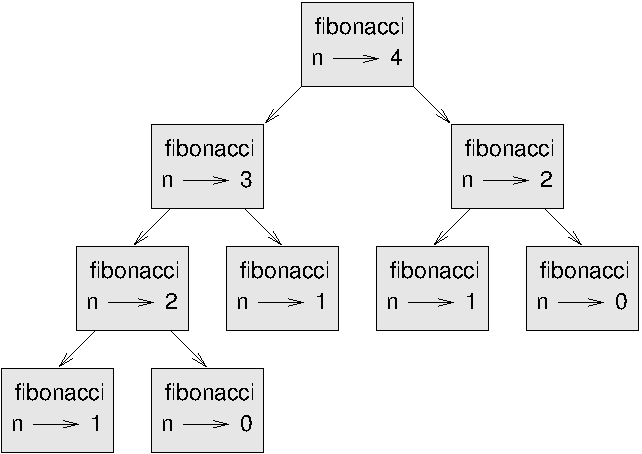
\includegraphics[scale=0.7]{../source/figs/fibonacci.pdf}}
\caption{Call graph.}
\label{fig.fibonacci}
\end{figure}

%🍁% A call graph shows a set of function frames, with lines connecting each
%🍁% frame to the frames of the functions it calls.  At the top of the
%🍁% graph, {\tt fibonacci} with {\tt n=4} calls {\tt fibonacci} with {\tt
%🍁% n=3} and {\tt n=2}.  In turn, {\tt fibonacci} with {\tt n=3} calls
%🍁% {\tt fibonacci} with {\tt n=2} and {\tt n=1}.  And so on.

调用图中列出了一系列函数栈帧, 每个栈帧之间通过线条与调用它的函数栈帧相连。
在图的顶端, \li{n = 4} 的 \li{fibonacci} 调用 \li{n = 3} 和 \li{n = 2} 的 \li{fibonacci} 。   接着,  \li{n = 3} 的 \li{fibonacci} 调用 \li{n = 2} 和 \li{n = 1} 的 \li{fibonacci}。   以此类推。

\index{function frame}  \index{frame}
\index{call graph}

%🍁% Count how many times {\tt fibonacci(0)} and {\tt fibonacci(1)} are
%🍁% called.  This is an inefficient solution to the problem, and it gets
%🍁% worse as the argument gets bigger.

数数 \li{fibonacci(0)} 和 \li{fibonacci(1)} 总共被调用了几次。
对该问题, 这不是一个高效的解, 并且随着实参的变大会变得更糟。

\index{memo}

%🍁% One solution is to keep track of values that have already been
%🍁% computed by storing them in a dictionary.  A previously computed value
%🍁% that is stored for later use is called a {\bf memo}.  Here is a
%🍁% ``memoized'' version of {\tt fibonacci}:

一个解决办法是保存已经计算过的值, 将它们存在一个字典中。
存储之前计算过的值以便今后使用, 它被称作 {\em 备忘录} (memo) 。
下面是使用备忘录 (memoized) 的 \li{fibonacci} 的实现:

\begin{lstlisting}
known = {0:0, 1:1}

def fibonacci(n):
    if n in known:
        return known[n]

    res = fibonacci(n-1) + fibonacci(n-2)
    known[n] = res
    return res
\end{lstlisting}

%
%🍁% {\tt known} is a dictionary that keeps track of the Fibonacci
%🍁% numbers we already know.  It starts with
%🍁% two items: 0 maps to 0 and 1 maps to 1.

\li{known} 是一个字典, 记录了我们已经计算过的斐波纳契数字。
它一开始包含两个项:0映射到0, 1映射到1。

%🍁% Whenever {\tt fibonacci} is called, it checks {\tt known}.
%🍁% If the result is already there, it can return
%🍁% immediately.  Otherwise it has to
%🍁% compute the new value, add it to the dictionary, and return it.

当 \li{fibonacci} 被调用时, 它先检查 \li{known} 。   如果结果存在, 则立即返回。   否则, 它必须计算新的值, 将其加入字典, 并返回它。

%🍁% If you run this version of {\tt fibonacci} and compare it with
%🍁% the original, you will find that it is much faster.

将两个版本的 \li{fibonacci} 函数比比看, 你就知道后者快了很多。


%🍁% \section{Global variables  |  全局变量}
\section{全局变量}

\index{global variable}  \index{variable!global}

%🍁% In the previous example, {\tt known} is created outside the function,
%🍁% so it belongs to the special frame called \verb"__main__".
%🍁% Variables in \verb"__main__" are sometimes called {\bf global}
%🍁% because they can be accessed from any function.  Unlike local
%🍁% variables, which disappear when their function ends, global variables
%🍁% persist from one function call to the next.

在前面的例子中, \li{known} 是在函数的外部创建的,
因此它属于被称作 \li{__main__} 的特殊帧。
因为 \li{__main__} 中的变量可以被任何函数访问, 它们也被称作 {\em 全局变量} (global) 。   与函数结束时就会消失的局部变量不同, 不同函数调用时全局变量一直都存在。

\index{flag}

%🍁% It is common to use global variables for {\bf flags}; that is,
%🍁% boolean variables that indicate (``flag'') whether a condition
%🍁% is true.  For example, some programs use
%🍁% a flag named {\tt verbose} to control the level of detail in the
%🍁% output:

全局变量普遍用作 {\em 标记} (flag); 就是说明(标记)一个条件是否为真的布尔变量。
例如, 一些程序使用一个被称作 \li{verbose} 的标记来控制输出的丰富程度:

\begin{lstlisting}
verbose = True

def example1():
    if verbose:
        print('Running example1')
\end{lstlisting}

%
%🍁% If you try to reassign a global variable, you might be surprised.
%🍁% The following example is supposed to keep track of whether the
%🍁% function has been called:

如果你试图对一个全局变量重新赋值, 结果可能出乎意料。
下面的例子本应该记录函数是否已经被调用过了

\index{reassignment}

\begin{lstlisting}
been_called = False

def example2():
    been_called = True         # WRONG
\end{lstlisting}

%
%🍁% But if you run it you will see that the value of \verb"been_called"
%🍁% doesn't change.  The problem is that {\tt example2} creates a new local
%🍁% variable named \verb"been_called".  The local variable goes away when
%🍁% the function ends, and has no effect on the global variable.

但是如果你运行它, 你会发现 \li{been_called} 的值并未发生改变。
问题在于 \li{example2} 生成了一个新的被称作 \li{been_called} 的局部变量。
当函数结束的时候, 该局部变量也消失了, 并且对全局变量没有影响。

\index{global statement}  \index{statement!global}
\index{declaration}

%🍁% To reassign a global variable inside a function you have to
%🍁% {\bf declare} the global variable before you use it:

要在函数内对全局变量重新赋值, 你必须在使用之前 {\em 声明} (declare) 该全局变量:

\begin{lstlisting}
been_called = False

def example2():
    global been_called
    been_called = True
\end{lstlisting}

%
%🍁% The {\bf global statement} tells the interpreter
%🍁% something like, ``In this function, when I say \verb"been_called", I
%🍁% mean the global variable; don't create a local one.''

\li{global} 语句 告诉编译器, ``在这个函数里, 当我说 \li{been_called} 时, 我指的是那个全局变量, 别生成局部变量''。

\index{update!global variable}  \index{global variable!update}

%🍁% Here's an example that tries to update a global variable:

下面是一个试图更新全局变量的例子:

\begin{lstlisting}
count = 0

def example3():
    count = count + 1          # WRONG
\end{lstlisting}

%
%🍁% If you run it you get:

一旦运行, 你会发现:

\index{UnboundLocalError}  \index{exception!UnboundLocalError}

\begin{lstlisting}
UnboundLocalError: local variable 'count' referenced before assignment
\end{lstlisting}

%
%🍁% Python assumes that {\tt count} is local, and under that assumption
%🍁% you are reading it before writing it.  The solution, again,
%🍁% is to declare {\tt count} global.

Python默认 \li{count} 是局部变量, 在这个假设下, 你这是在未写入任何东西前就试图读取。
解决方法还是声明 \li{count} 是全局变量。

\index{counter}

\begin{lstlisting}
def example3():
    global count
    count += 1
\end{lstlisting}

%
%🍁% If a global variable refers to a mutable value, you can modify
%🍁% the value without declaring the variable:

如果全局变量是可变的, 你可以不加声明地修改它:

\index{mutability}

\begin{lstlisting}
known = {0:0, 1:1}

def example4():
    known[2] = 1
\end{lstlisting}

%
%🍁% So you can add, remove and replace elements of a global list or
%🍁% dictionary, but if you want to reassign the variable, you
%🍁% have to declare it:

因此你可以增加、删除和替代全局列表或者字典的元素,
但是如果你想对变量重新赋值, 你必须声明它:

\begin{lstlisting}
def example5():
    global known
    known = dict()
\end{lstlisting}

%
%🍁% Global variables can be useful, but if you have a lot of them,
%🍁% and you modify them frequently, they can make programs
%🍁% hard to debug.

全局变量有时是很有用的, 但如果你的程序中有很多全局变量, 而且修改频繁,
这样会增加程序调试的难度。

%🍁% \section{Debugging  |  调试}
\section{调试}
\index{debugging}

%🍁% As you work with bigger datasets it can become unwieldy to
%🍁% debug by printing and checking the output by hand.  Here are some
%🍁% suggestions for debugging large datasets:

当你操作较大的数据集时, 通过打印并手工检查数据来调试很不方便。
下面是针对调试大数据集的一些建议:

%🍁% \begin{description}
%🍁%
%🍁% \item[Scale down the input:] If possible, reduce the size of the
%🍁% dataset.  For example if the program reads a text file, start with
%🍁% just the first 10 lines, or with the smallest example you can find.
%🍁% You can either edit the files themselves, or (better) modify the
%🍁% program so it reads only the first {\tt n} lines.
%🍁%
%🍁% If there is an error, you can reduce {\tt n} to the smallest
%🍁% value that manifests the error, and then increase it gradually
%🍁% as you find and correct errors.
%🍁%
%🍁% \item[Check summaries and types:] Instead of printing and checking the
%🍁% entire dataset, consider printing summaries of the data: for example,
%🍁% the number of items in a dictionary or the total of a list of numbers.
%🍁%
%🍁% A common cause of runtime errors is a value that is not the right
%🍁% type.  For debugging this kind of error, it is often enough to print
%🍁% the type of a value.
%🍁%
%🍁% \item[Write self-checks:]  Sometimes you can write code to check
%🍁% for errors automatically.  For example, if you are computing the
%🍁% average of a list of numbers, you could check that the result is
%🍁% not greater than the largest element in the list or less than
%🍁% the smallest.  This is called a ``sanity check'' because it detects
%🍁% results that are ``insane''.
%🍁%
%🍁% \index{sanity check}  \index{consistency check}
%🍁%
%🍁% Another kind of check compares the results of two different
%🍁% computations to see if they are consistent.  This is called a
%🍁% ``consistency check''.
%🍁%
%🍁% \item[Format the output:] Formatting debugging output
%🍁% can make it easier to spot an error.  We saw an example in
%🍁% Section~\ref{factdebug}.  The {\tt pprint} module provides
%🍁% a {\tt pprint} function that displays built-in types in
%🍁% a more human-readable format ({\tt pprint} stands for
%🍁% ``pretty print'').
%🍁%
%🍁% \index{pretty print}  \index{pprint module}
%🍁% \index{module!pprint}
%🍁%
%🍁% \end{description}

\begin{description}

\item[缩小输入(Scale down the input):] 如果可能, 减小数据集合的大小。
    例如, 如果程序读入一个文本文件, 从前10行开始分析, 或是找到更小的样例。
    你可以选择编辑读入的文件, 或是(最好)修改程序使它只读入前 \li{n} 行。

    如果出错了, 你可以将 \li{n} 缩小为会导致该错误的最小值, 然后在查找和解决错误的同时, 逐步增加 n 的值。

\item[检查摘要和类型(Check summaries and types):] Instea考虑打印数据的摘要, 而不是打印并检查全部数据集合:
    例如, 字典中项的数目或者数字列表的总和。

    运行时错误的一个常见原因, 是值的类型不正确。   为了调试此类错误, 打印值的类型通常就足够了。

\item[编写自检代码(Write self-checks):]  有时你可以写代码来自动检查错误。   例如, 如果你正在计算数字列表的平均数, 你可以检查其结果是不是大于列表中最大的元素, 或者小于最小的元素。   这被称 作``合理性检查'', 因为它能检测出``不合理的''结果。

\index{sanity check}  \index{consistency check}

另一类检查是比较两个不同计算的结果, 来看一下它们是否一致。  这被称作 ``一致性检查''。

\item[格式化输出(Format the output):] 格式化调试输出能够更容易定位一个错误。   我们在 \ref{factdebug} 一节中看过一个示例。   \li{pprint} 模块提供了一个 \li{pprint} 函数, 它可以更可读的格式显示内建类型( \li{pprint} 代表 ``pretty print'')。

\index{pretty print}  \index{pprint module}
\index{module!pprint}

\end{description}

%🍁% Again, time you spend building scaffolding can reduce
%🍁% the time you spend debugging.

重申一次, 你花在搭建脚手架上的时间能减少你花在调试上的时间。

\index{scaffolding}


%🍁% \section{Glossary  |  术语表}
\section{术语表}

\begin{description}

%🍁% \item[mapping:] A relationship in which each element of one set
%🍁% corresponds to an element of another set.
%🍁%
%🍁% \index{mapping}

\item[映射 (mapping):] 一个集合中的每个元素对应另一个集合中的一个元素的关系。

\index{mapping}

%🍁% \item[dictionary:] A mapping from keys to their
%🍁% corresponding values.
%🍁%
%🍁% \index{dictionary}

\item[字典 (dictionary):] 将键映射到对应值的映射。

\index{dictionary}

%🍁% \item[key-value pair:] The representation of the mapping from
%🍁% a key to a value.
%🍁%
%🍁% \index{key-value pair}

\item[键值对 (key-value pair):] 键值之间映射关系的呈现形式。

\index{key-value pair}

%🍁% \item[item:] In a dictionary, another name for a key-value
%🍁%   pair.
%🍁%
%🍁% \index{item!dictionary}

\item[项 (item):] 在字典中, 这是键值对的另一个名称。

\index{item!dictionary}

%🍁% \item[key:] An object that appears in a dictionary as the
%🍁% first part of a key-value pair.
%🍁%
%🍁% \index{key}

\item[键 (key):] 字典中作为键值对第一部分的对象。

%🍁% \index{key}
%🍁%
%🍁% \item[value:] An object that appears in a dictionary as the
%🍁% second part of a key-value pair.  This is more specific than
%🍁% our previous use of the word ``value''.
%🍁%
%🍁% \index{value}

\item[值 (value):] 字典中作为键值对第二部分的对象。  它比我们之前所用的``值''一词更具体。

\index{value}

%🍁% \item[implementation:] A way of performing a computation.
%🍁%
%🍁% \index{implementation}

\item[实现 (implementation):] 执行计算的一种形式。

\index{implementation}

%🍁% \item[hashtable:] The algorithm used to implement Python
%🍁% dictionaries.
%🍁%
%🍁% \index{hashtable}

\item[哈希表 (hashtable):] 用来实现Python字典的算法。

\index{hashtable}

%🍁% \item[hash function:] A function used by a hashtable to compute the
%🍁% location for a key.
%🍁%
%🍁% \index{hash function}

\item[哈希函数 (hash function):] 哈希表用来计算键的位置的函数。

\index{hash function}

%🍁% \item[hashable:] A type that has a hash function.  Immutable
%🍁% types like integers,
%🍁% floats and strings are hashable; mutable types like lists and
%🍁% dictionaries are not.
%🍁%
%🍁% \index{hashable}

\item[可哈希的 (hashable):] 具备哈希函数的类型。  诸如整数、浮点数和字符串这样的不可变类型是可哈希的;诸如列表和字典这样的可变对象是不可哈希的。

\index{hashable}

%🍁% \item[lookup:] A dictionary operation that takes a key and finds
%🍁% the corresponding value.
%🍁%
%🍁% \index{lookup}

\item[查找 (lookup):] 接受一个键并返回相应值的字典操作。

\index{lookup}

%🍁% \item[reverse lookup:] A dictionary operation that takes a value and finds
%🍁% one or more keys that map to it.
%🍁%
%🍁% \index{reverse lookup}

\item[逆向查找 (reverse lookup):] 接受一个值并返回一个或多个映射至该值的键的字典操作。

\index{reverse lookup}

%🍁% \item[raise statement:]  A statement that (deliberately) raises an exception.
%🍁%
%🍁% \index{raise statement}  \index{statement!raise}

\item[raise语句:]  专门印发异常的一个语句。

\index{raise statement}  \index{statement!raise}

%🍁% \item[singleton:] A list (or other sequence) with a single element.
%🍁% \index{singleton}

\item[单元素集合 (singleton):] 只有一个元素的列表(或其他序列)。
\index{singleton}

%🍁% \item[call graph:] A diagram that shows every frame created during
%🍁% the execution of a program, with an arrow from each caller to
%🍁% each callee.
%🍁%
%🍁% \index{call graph}  \index{diagram!call graph}

\item[调用图 (call graph):] 绘出程序执行过程中创建的每个栈帧的调用图, 其中的箭头从调用者指向被调用者。

\index{call graph}  \index{diagram!call graph}

%🍁% \item[memo:] A computed value stored to avoid unnecessary future
%🍁% computation.
%🍁%
%🍁% \index{memo}

\item[备忘录 (memo):] 一个存储的计算值, 避免之后进行不必要的计算。

\index{memo}

%🍁% \item[global variable:]  A variable defined outside a function.  Global
%🍁% variables can be accessed from any function.
%🍁%
%🍁% \index{global variable}

\item[全局变量 (global variable):]  在函数外部定义的变量。  任何函数都可以访问全局变量。

\index{global variable}

%🍁% \item[global statement:]  A statement that declares a variable name
%🍁% global.
%🍁%
%🍁% \index{global statement}  \index{statement!global}

\item[global语句:]  将变量名声明为全局变量的语句。

\index{global statement}  \index{statement!global}

%🍁% \item[flag:] A boolean variable used to indicate whether a condition
%🍁% is true.
%🍁%
%🍁% \index{flag}

\item[标记 (flag):] 用于说明一个条件是否为真的布尔变量。

\index{flag}

%🍁% \item[declaration:] A statement like {\tt global} that tells the
%🍁% interpreter something about a variable.
%🍁%
%🍁% \index{declaration}

\item[声明 (declaration):] 类似 \li{global} 这种告知解释器如何处理变量的语句。

\index{declaration}

\end{description}



%🍁% \section{Exercises  |  练习}
\section{练习}

\begin{exercise}
\label{wordlist2}

\index{set membership}  \index{membership!set}

%🍁% Write a function that reads the words in {\tt words.txt} and
%🍁% stores them as keys in a dictionary.  It doesn't matter what the
%🍁% values are.  Then you can use the {\tt in} operator
%🍁% as a fast way to check whether a string is in
%🍁% the dictionary.
%🍁%
%🍁% If you did Exercise~\ref{wordlist1}, you can compare the speed
%🍁% of this implementation with the list {\tt in} operator and the
%🍁% bisection search.

编写一函数, 读取 {\em \li{words.txt}} 中的单词并存储为字典中的键。  值是什么无所谓。
然后, 你可以使用 {\em \li{in}} 操作符检查一个字符串是否在字典中。

如果你做过 练习~\ref{wordlist1} , 可以比较一下 {\em \li{in}} 操作符和二分查找的速度。

\end{exercise}


\begin{exercise}
\label{setdefault}

%🍁% Read the documentation of the dictionary method {\tt setdefault}
%🍁% and use it to write a more concise version of \verb"invert_dict".
%🍁% Solution: \url{http://thinkpython2.com/code/invert_dict.py}.

查看字典方法 {\em \li{setdefault}} 的文档, 并使用该方法写一个更简洁的 {\em \li{invert_dict}}。

\index{setdefault method}  \index{method!setdefault}

\end{exercise}


\begin{exercise}
%🍁% Memoize the Ackermann function from Exercise~\ref{ackermann} and see if
%🍁% memoization makes it possible to evaluate the function with bigger
%🍁% arguments.  Hint: no.
%🍁% Solution: \url{http://thinkpython2.com/code/ackermann_memo.py}.

将 练习~{\em \ref{ackermann}} 中的 {\em Ackermann} 函数备忘录化\footnote{memoization}, 看看备忘录化是否可以支持解决更大的参数。   没有提示!

\href{http://thinkpython2.com/code/ackermann_memo.py}{参考答案}
\index{Ackermann function}  \index{function!ack}

\end{exercise}

\begin{exercise}

\index{duplicate}

%🍁% If you did Exercise~\ref{duplicate}, you already have
%🍁% a function named \verb"has_duplicates" that takes a list
%🍁% as a parameter and returns {\tt True} if there is any object
%🍁% that appears more than once in the list.
%🍁%
%🍁% Use a dictionary to write a faster, simpler version of
%🍁% \verb"has_duplicates".
%🍁% Solution: \url{http://thinkpython2.com/code/has_duplicates.py}.

如果你做了 练习~{\em \ref{duplicate}} , 你就已经有了一个叫 {\em \li{has_duplicates}} 的函数, 它接受一个列表作为参数, 如果其中有某个对象在列表中出现不止一次就返回 {\em \li{True}}。

用字典写个更快、更简单的版本。

\href{http://thinkpython2.com/code/has_duplicates.py}{参考答案}


\end{exercise}


\begin{exercise}
\label{exrotatepairs}

\index{letter rotation}  \index{rotation!letters}

%🍁% Two words are ``rotate pairs'' if you can rotate one of them
%🍁% and get the other (see \verb"rotate_word" in Exercise~\ref{exrotate}).
%🍁%
%🍁% Write a program that reads a wordlist and finds all the rotate
%🍁% pairs.  Solution: \url{http://thinkpython2.com/code/rotate_pairs.py}.

两个单词如果反转其中一个就会得到另一个, 则被称作 ``反转对''(参见 练习~{\em \ref{exrotate}} 中的 {\em \li{rotate_word}} 。

编写一程序, 读入单词表并找到所有反转对。

\href{http://thinkpython2.com/code/rotate_pairs.py}{参考答案}

\end{exercise}


\begin{exercise}

\index{Car Talk}  \index{Puzzler}

%🍁% Here's another Puzzler from {\em Car Talk}
%🍁% (\url{http://www.cartalk.com/content/puzzlers}):

下面是取自 {\em Car Talk} 的另一个字\href{http://www.cartalk.com/content/puzzlers}{谜题}:

%🍁% \begin{quote}
%🍁% This was sent in by a fellow named Dan O'Leary. He came upon a common
%🍁% one-syllable, five-letter word recently that has the following unique
%🍁% property. When you remove the first letter, the remaining letters form
%🍁% a homophone of the original word, that is a word that sounds exactly
%🍁% the same. Replace the first letter, that is, put it back and remove
%🍁% the second letter and the result is yet another homophone of the
%🍁% original word. And the question is, what's the word?
%🍁%
%🍁% Now I'm going to give you an example that doesn't work. Let's look at
%🍁% the five-letter word, `wrack.' W-R-A-C-K, you know like to `wrack with
%🍁% pain.' If I remove the first letter, I am left with a four-letter
%🍁% word, 'R-A-C-K.' As in, `Holy cow, did you see the rack on that buck!
%🍁% It must have been a nine-pointer!' It's a perfect homophone. If you
%🍁% put the `w' back, and remove the `r,' instead, you're left with the
%🍁% word, `wack,' which is a real word, it's just not a homophone of the
%🍁% other two words.
%🍁%
%🍁% But there is, however, at least one word that Dan and we know of,
%🍁% which will yield two homophones if you remove either of the first two
%🍁% letters to make two, new four-letter words. The question is, what's
%🍁% the word?
%🍁% \end{quote}

\begin{quote}

这是来自一位名叫 {\em Dan O'Leary} 的朋友的分享。  他有一次碰到了一个常见的单音节、有五个字母的单词, 它具备以下独特的特性。  当你移除第一个字母时, 剩下的字母组成了原单词的同音词, 即发音完全相同的单词。  将第一个字母放回, 然后取出第二个字母, 结果又是原单词的另一个同音词。  那么问题来了, 这个单词是什么?

接下来我给大家举一个不满足要求的例子。  我们来看一个五个字母的单词 {\em ``wrack''}。  W-R-A-C-K, 常用短句为  {\em ``wrack with pain''}。   如果我移除第一个字母, 就剩下了一个四个字母的单词  {\em ``R-A-C-K''}。  可以这么用,  {\em ``Holy cow, did you see the rack on that buck! It must have been a nine-pointer!''} 它是一个完美的同音词。  如果你把  {\em ``w''} 放回去, 移除  {\em ``r''},  你得到的单词是  {\em ``wack''} 。   这是一个真实的单词, 但并不是前两个单词的同音词。

不过, 我们和 {\em Dan} 知道至少有一个单词是满足这个条件的, 即移除前两个字母中的任意一个, 将会得到两个新的由四个字母组成的单词, 而且发音完全一致。  那么这个单词是什么呢?

\end{quote}

\index{homophone}  \index{reducible word}
\index{word, reducible}

%🍁% You can use the dictionary from Exercise~\ref{wordlist2} to check
%🍁% whether a string is in the word list.

你可以使用 练习~{\em \ref{wordlist2}} 中的字典检查某字符串是否出现在单词表中。

%🍁% To check whether two words are homophones, you can use the CMU
%🍁% Pronouncing Dictionary.  You can download it from
%🍁% \url{http://www.speech.cs.cmu.edu/cgi-bin/cmudict} or from
%🍁% \url{http://thinkpython2.com/code/c06d} and you can also download
%🍁% \url{http://thinkpython2.com/code/pronounce.py}, which provides a function
%🍁% named \verb"read_dictionary" that reads the pronouncing dictionary and
%🍁% returns a Python dictionary that maps from each word to a string that
%🍁% describes its primary pronunciation.

你可以使用CMU发音字典检查两个单词是否为同音词。  从 \href{http://www.speech.cs.cmu.edu/cgi-bin/cmudict}{这里} 或 \href{http://thinkpython2.com/code/c06d}{这里} 下载。   你还可以下载\href{http://thinkpython2.com/code/pronounce.py}{ 这个脚本}, 其中提供了一个名叫 \li{read_dictionary} 的函数, 可以读取发音字典, 并返回一个将每个单词映射至描述其主要梵音的字符串的Python字典。

%🍁% Write a program that lists all the words that solve the Puzzler.
%🍁% Solution: \url{http://thinkpython2.com/code/homophone.py}.

编写一个程序, 找到满足字谜题条件的所有单词。

\href{http://thinkpython2.com/code/homophone.py}{参考答案}

\end{exercise}
